\subsection{Adamant}
Adamant ist ein kostenloses Open-Source Tool zum gemeinsamen Management von Sicherheitsanforderungen. Dazu unterstützt es die Modellierung von Requirements auf Grundlage von zum Beispiel dem BSI-Grundschutzkatalog.\cite{adamant}\\ 
Zum Testen stand nur eine Live-Demo der Software zur Verfügung, so dass das Beispiel der Hochschule nicht nach modelliert werden konnte. Die Bewertung gründet sich damit auf den in der Live-Demo beispielhaft zur Verfügung gestellten Daten.\\

\begin{table}[h!bt]
	%\centering
	\begin{tabular}{|p{0.5\textwidth}|p{0.5\textwidth}|}
		\hline 
		Kriterium & Bewertung\\ 
		\hline 
		\textbf{GUI}& \\
		\hline
		Wizard & 0\\
		\hline 
		Infrastrukturdarstellung & 8 \\
		\hline 
		Netzpläne & 0 \\
		\hline 
		Prozessflüsse & 0 \\
		\hline 
		Schnelles Einpflegen von Änderungen & 8 \\
		\hline
		\textbf{Objektrelationen} & \\
		\hline 
		Doppelseitige Verlinkungen & 8 \\
		\hline 
		Vererbung & 0 \\
		\hline 
		Gruppierungen & 0 \\
		\hline 
		\textbf{Funktionalität} &\\
		\hline 
		Aktuelle BSI-Standards & 5 \\
		\hline  
		Erweiterbarkeit der Klassifizierungen & 7 \\
		\hline 
		Individuelle Beschreibungen & 8 \\
		\hline 
		Sicherheitsverstöße markieren & 8 \\
		\hline
		Bewertung des Sicherheitsstatus & 4 \\
		\hline
		Export von Berichten & 6 \\
		\hline
		BSI-Toolimport & 0 \\
		\hline
		Sicherheit des Tools an sich & 0 \\
		\hline
		Risikobewertung & 0 \\
		\hline
		\textbf{System}&  \\
		\hline
		Verteiltes Arbeiten & 5 \\
		\hline
		Rechtevergabe & 0 \\
		\hline
		Kosten & 7 \\
		\hline
		Support & 2 \\
		\hline
		Zertifizierung & 0 \\
		\hline
		Dokumentation & 0 \\
		\hline
		Marktpräsenz & 0 \\
		\hline
		Spezielle Zielgruppe & 0 \\
		\hline
		Pflege/Weiterentwicklung & 8 \\
		\hline
		\multicolumn{2}{c}{}\\
		\hline
		\textbf{Gesamt} & \\
		\hline
		Hochschuleinsatz & 35\%\\
		\hline
		Lehre & rund 43\%\\
		\hline
	\end{tabular} 
	\caption{Bewertung: Adamant}
	\label{tab:BewertungAdamant}
\end{table}
Für die Kriterien Wizard, Netzpläne und Prozessflüsse unter dem Punkt GUI wurden jeweils 0 Punkte vergeben, da das Tool nicht über Wizards zur Projekterstellung oder Erstellung zum Beispiel eines zu schützenden Wertes oder Risikos verfügt beziehungsweise keine Netzpläne oder Prozessflüsse modelliert und dargestellt werden können. Die Infrastrukturdarstellung erhielt 8 Punkte, da eine gute hierarchisch organisierte Übersicht über die angelegten Assets abrufbar ist. Punktabzug gab es hier nur weil die Navigation in dieser Hierarchie etwas umständlich ist. Auch erhielt das Kriterium der schnellen Einarbeitung von Änderungen ein Bewertung von 8, da es über die Metadaten (Meta Data) recht einfach ist alle relevante Objekte wie die zu schützenden Werte (Assets), die Risiken (Risks), die Quellen (Soucres) die für ein Requirement hinterlegt werden können und die zuständigen Stellen (Stakeholder) zu editieren oder anzulegen.\\
\begin{figure}[h!bp]
\label{fig:admantHierarchie}
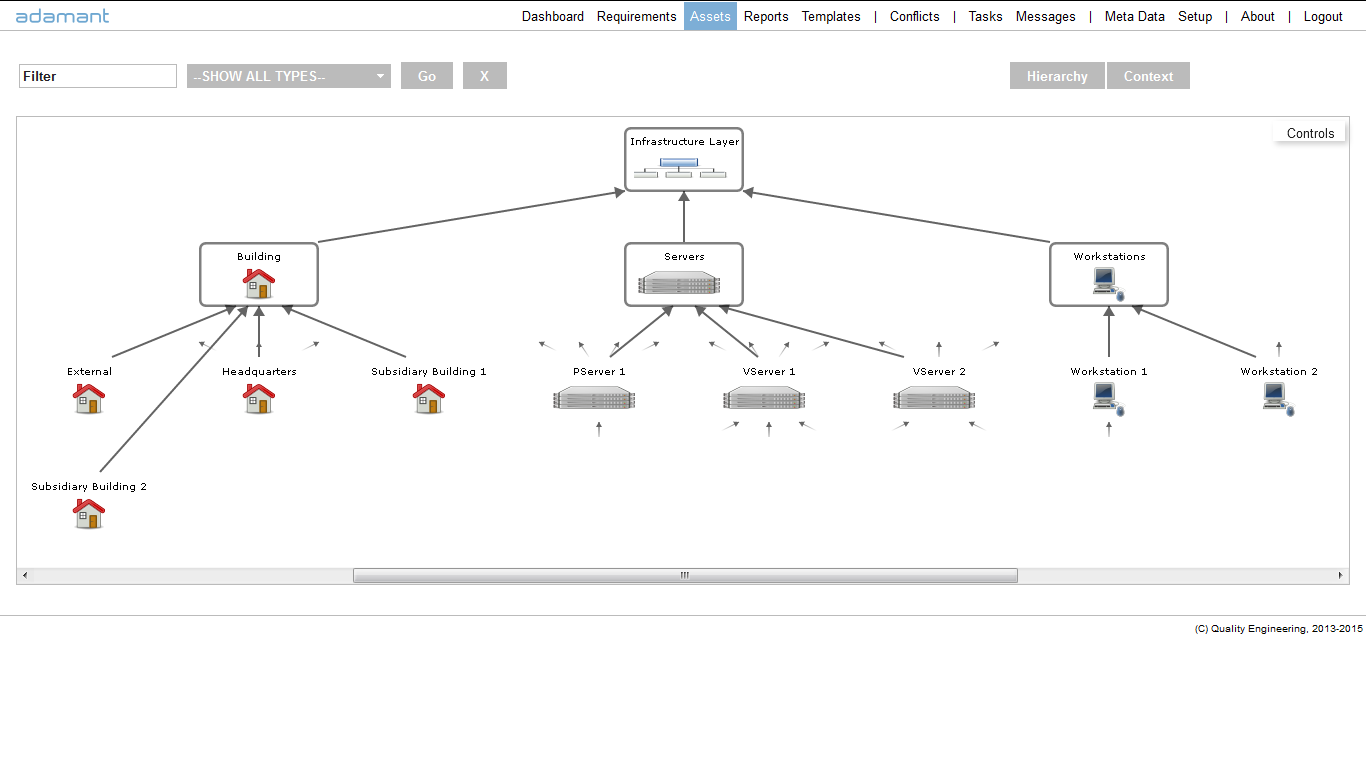
\includegraphics[scale=0.40]{images/adamant_hierarchie.png} 
\caption{Hierarchische Darstellung der Infrastruktur mit Adamant}
\end{figure}\\
Bei den Objektrelationen erhielt die doppelseitigen Verlinkungen 8 Punkte, da diese über die Metadaten (Meta Data) einfach zwischen den Assets hinterlegt werden können. Punktabzug gab es hier da nicht zu erkennen war, dass sich diese Verlinkungen auf die Sicherheitsbewertung ausgewirkt haben. Hingegen wurden die Vererbung und die Gruppierung mit 0 Punkten bewertet, da diese nicht möglich sind.\\
Unter den Funktionalitäten des Tools wurde die Erweiterbarkeit der Klassifizierungen mit 7 Punkten bewertet, weil sowohl die Erfüllungs- als auch die Revalidierungsmodelle sowie die Prioritäten um eigene Klassen erweiterte werden können. Die individuellen Beschreibungen erhielten 8 Punkte, da sie für alle Objekte hinterlegt werden können, sowohl für einzelne Assets oder Risiken als auch für die Report und die Requirements. Der Export von Berichten wurde mit 6 Punkten bewertet, weil es zwar möglich ist Reports zu erstellen und auch eigene zu definieren, diese aber recht wenig aussagekräftig sind. Für die aktuellen BSI-Standards gab es 5 Punkte, da zum Zeitpunkt der Analyse die Standards von 2013 als Grundlage dienten, aber keine Möglichkeit erkenntlich war neue Standards einzupflegen, wie zum Beispiel eine Update-Funktion. Es kann aber auch möglich sein das eine derartige Funktion in der Live-Demo nur deaktiviert ist und somit nicht angezeigt wird. Der GS-Tool Import erhielt eine Bewertung von 0 Punkten, da keine Funktion zum Importieren von Modellen aus dem Grundschutz-Tool des BSI vorhanden ist. Die Markierung von Sicherheitsverstößen wurde mit 8 Punkten bewertet und die Bewertung des Sicherheitsstatus mit 4 Punkten, da das Programm nur jene der selbsterstellen Requirements markiert, die nicht erfüllt sind oder revalidiert werden müssen. Die Sicherheit des Tools an sich erhielt eine Bewertung von 0 Punkten, da es keine Angaben über eine Verschlüsselung der gespeicherten Daten oder eine andere Schutzmaßnahme für die Daten gibt. Die zusätzliche Risikobewertung wurde mit 0 Punkten bewertet, weil das Programm eine solche nicht unterstützt.\\
\begin{figure}[h!bp]
\label{fig:admantReports}
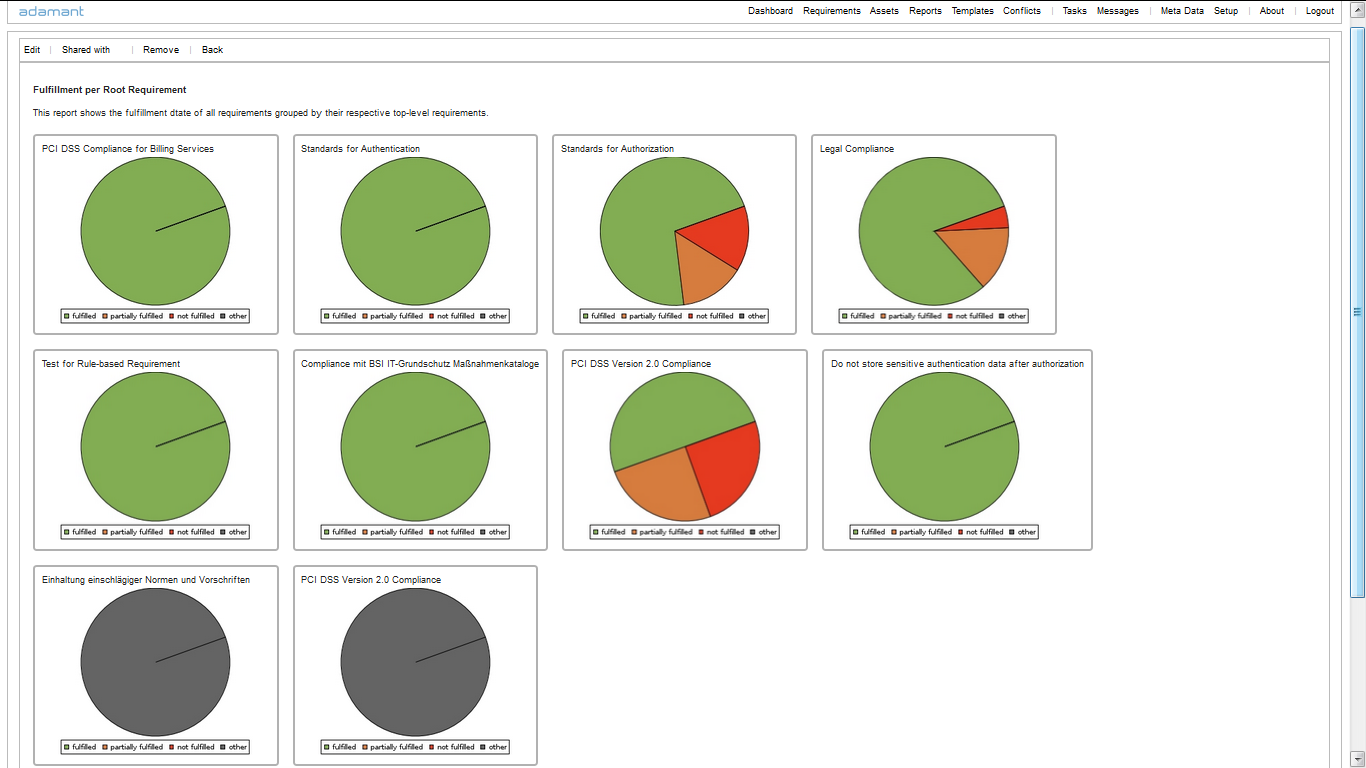
\includegraphics[scale=0.40]{images/adamant_reports.png} 
\caption{Mit Adamant erstellter Erfüllungsbericht für Sicherheitsanforderungen}
\end{figure}
Unter dem Punkt System wurde das verteilte Arbeiten mit einer Bewertung von  5 versehen, da es webbasiert ist und für das gemeinsame Entwickeln der Sicherheitsanforderungen konzipiert ist. Punktabzug gab es weil Softwareseitig, in der Live-Demo, keine Rechtevergabe möglich war. Daher auch die 0 Punkte für das Kriterium Rechtevergabe. Eine Zertifizierung durch Einsatz dieses Programms ist nicht möglich, daher gab es auch hierfür 0 Punkte. Auch für Marktpräsenz und Nutzerkreis gab es 0 Punkte, da keine Referenzen gefunden werden konnten, dass dieses Programm produktiv im Einsatz ist und kein bestimmter Nutzerkreis aus zu machen ist. Auch die Dokumentation erhielt 0 Punkte, weil keine gefunden werden konnte. Der herrunterladbaren Source-Code soll auch eine Dokumentation beiliegen, was leider nicht überprüft werden konnte, da der Versuch des Download immer mit einer Fehlermeldung endete. Für die Kosten wurden 7 Punkte vergeben, weil es sich um ein kostenloses Open-Soucre Tool handelt, welches noch weiterentwickelt wird. Deshalb erhielt auch Pflege/Weiterentwicklung 8 Punkte.\\
